% =============================================================================
%  Desenvolvimento de Arvore-B em Memoria Secundaria
%  Slides Beamer, em pt-br. Estrutura segue o "Modelo de apresentacao PPT" do
%  enunciado (AED-PG-2026-Trabalho.pdf): 10 slides + alguns extras.
%
%  COMPILAR com `make slides`, que usa o TeX Live instalado LOCALMENTE no
%  projeto (./.texlive, via `make tex-install`) -- sem mise nem TeX de sistema.
%  Duas passadas resolvem TOC/navegacao.
%
%  Dados das tabelas: data/resultados_experimentos.csv e
%  data/reuso_comparacao.csv (gerados por `make run_experiments`).
% =============================================================================
\documentclass[aspectratio=169,11pt]{beamer}

\usetheme{default}

\usepackage[T1]{fontenc}
\usepackage[utf8]{inputenc}
\usepackage[portuguese]{babel}
\usepackage{listings}
\usepackage{xcolor}
\usepackage{booktabs}
\usepackage{graphicx}
\graphicspath{{img/}}

% ---- Paleta: azul do PPTX de referencia (4472C4) ---------------------------
\definecolor{btblue}{HTML}{4472C4}
\definecolor{btorange}{HTML}{ED7D31}
\definecolor{btgray}{HTML}{595959}
\definecolor{codebg}{HTML}{F4F6FB}
\definecolor{termbg}{HTML}{1E1E1E}
\definecolor{termgreen}{HTML}{4EC9B0}

% ---- Visual limpo (estilo metropolis com tema nativo, compila no pdflatex) --
\setbeamertemplate{navigation symbols}{}
\setbeamertemplate{footline}[frame number]
\setbeamercolor{frametitle}{bg=btblue,fg=white}
\setbeamercolor{title}{fg=btblue}
\setbeamercolor{structure}{fg=btblue}
\setbeamercolor{block title}{bg=btblue!18,fg=btblue!75!black}
\setbeamercolor{block body}{bg=btblue!6}
\setbeamercolor{alerted text}{fg=btblue}
\setbeamerfont{frametitle}{series=\bfseries}
\setbeamertemplate{blocks}[rounded][shadow=false]
\setbeamertemplate{itemize items}[circle]

% Barra de titulo ocupando a largura inteira (look metropolis).
\setbeamertemplate{frametitle}{%
  \nointerlineskip%
  \begin{beamercolorbox}[wd=\paperwidth,sep=9pt]{frametitle}%
    \usebeamerfont{frametitle}\insertframetitle%
  \end{beamercolorbox}%
}

% Slides divisores de secao (metropolis-like).
\AtBeginSection[]{%
  \begin{frame}[plain]
    \centering\vfill
    {\usebeamercolor[fg]{title}\Large\bfseries\insertsectionhead}
    \vfill
  \end{frame}%
}

% ---- Estilo dos trechos de codigo C++ --------------------------------------
\lstdefinestyle{cpp}{
  language=C++,
  basicstyle=\ttfamily\footnotesize,
  keywordstyle=\color{btblue}\bfseries,
  commentstyle=\color{btgray}\itshape,
  stringstyle=\color{btorange},
  backgroundcolor=\color{codebg},
  frame=single,
  rulecolor=\color{btblue!40},
  framexleftmargin=4pt,
  xleftmargin=6pt,
  xrightmargin=6pt,
  showstringspaces=false,
  breaklines=true,
  columns=fullflexible,
  keepspaces=true,
  aboveskip=4pt,
  belowskip=2pt,
}
\lstset{style=cpp}

% ---- Estilo "terminal" p/ os prints da interface (saida real do main.exe) ---
\lstdefinestyle{terminal}{
  basicstyle=\ttfamily\scriptsize\color{white},
  backgroundcolor=\color{termbg},
  frame=single,
  rulecolor=\color{termbg},
  framexleftmargin=3pt,
  xleftmargin=5pt,
  xrightmargin=5pt,
  showstringspaces=false,
  breaklines=true,
  columns=fullflexible,
  keepspaces=true,
  aboveskip=4pt,
  belowskip=2pt,
}

% ---- Metadados -------------------------------------------------------------
\title{Desenvolvimento de Árvore-B em Memória Secundária}
\subtitle{Trabalho de implementação e análise de desempenho}
\author{Caio Uehara \and Yuri Calzzani \and Igor Felipe}
\institute{PPGCA --- DCM \\ Algoritmos e Estruturas de Dados \\[2pt]
  \footnotesize Docente: Prof. Dr. José Augusto Baranauskas}
\date{}

\begin{document}

% ===== Slide 1: Capa ========================================================
{
\setbeamertemplate{footline}{}
\begin{frame}[plain]
  \titlepage
\end{frame}
}

% ===== Agenda (extra) =======================================================
\begin{frame}{Agenda}
  \tableofcontents
\end{frame}

% ###########################################################################
\section{Decisões e Arquitetura}
% ###########################################################################

% ===== Slide 2: Decisoes de implementacao ===================================
\begin{frame}{Decisões de Implementação}
  \begin{columns}[T,onlytextwidth]
    \begin{column}{0.48\textwidth}
      \begin{block}{Armazenamento da raiz}
        Mantida de forma \alert{dupla}:
        \begin{itemize}
          \item em memória, no atributo \texttt{rootID};
          \item em disco, no registro \texttt{0} (cabeçalho).
        \end{itemize}
        O cabeçalho é reescrito em 4 momentos: \emph{criação}, \emph{split},
        \emph{colapso} da raiz e \emph{carregamento}.
      \end{block}
    \end{column}
    \begin{column}{0.48\textwidth}
      \begin{block}{Reaproveitamento de nós --- \alert{sim}}
        \begin{itemize}
          \item \textbf{Estrutura:} lista de livres (``lixeira''), topo no
            \texttt{A[1]} do cabeçalho, encadeada pelo \texttt{A[0]} de cada
            registro livre.
          \item \textbf{Como:} \texttt{freeNode()} empilha o nó removido;
            \texttt{allocateNode()} recicla antes de crescer o arquivo.
        \end{itemize}
      \end{block}
    \end{column}
  \end{columns}
\end{frame}

% ===== Armazenamento em disco (extra; reforca o requisito de mem. secundaria)=
\begin{frame}[fragile]{Armazenamento estritamente em memória secundária}
  Cada nó é um registro de \alert{tamanho fixo} $(2M+3)\cdot\texttt{sizeof(int)}$,
  lido/escrito \alert{um por vez} por \emph{seek} + \emph{struct} (sem cache de
  vários nós em RAM) --- atende ao requisito do enunciado.
  \begin{lstlisting}
template <int M>
struct BTreeNode { int numKeys; int K[M+1]; int A[M+1]; };

file.seekg(id * sizeof(BTreeNode<M>), std::ios::beg); // 1 no
file.read ((char*)(&node), sizeof(BTreeNode<M>));     // 1 registro
  \end{lstlisting}
\end{frame}

% ===== Slide 3: Metodos implementados =======================================
\begin{frame}{Métodos Implementados}
  \begin{columns}[T,onlytextwidth]
    \begin{column}{0.5\textwidth}
      \begin{block}{\texttt{BTree<M>}}
        \footnotesize
        \texttt{search}, \texttt{insert}, \texttt{split}, \texttt{remove},
        \texttt{removeRecursive}, \texttt{borrowFromLeft/Right},
        \texttt{mergeChildren}, \texttt{loadFromFile}, \texttt{getHeight}.
      \end{block}
      \begin{block}{\texttt{BTreeNode}}
        \footnotesize
        \texttt{findIndex(key)} localiza a chave ou o ponto de inserção.
      \end{block}
    \end{column}
    \begin{column}{0.5\textwidth}
      \begin{block}{\texttt{DiskManager} (contador de I/O)}
        \footnotesize
        \texttt{incrementRead/Write}, \texttt{getReadCount/WriteCount},
        \texttt{resetCounters}, \texttt{getFileSize}.
      \end{block}
      \begin{block}{Módulo \texttt{Display}}
        \footnotesize
        \texttt{displayTree}, \texttt{displayLevelOrder}, \texttt{dumpFile},
        \texttt{displaySearchResult}. \emph{(lógica e visualização separadas.)}
      \end{block}
    \end{column}
  \end{columns}
\end{frame}

% ###########################################################################
\section{Demonstração}
% ###########################################################################

% ===== Print de codigo 1: reaproveitamento de nos ===========================
\begin{frame}[fragile]{Caso de uso em código: reaproveitamento de nós}
  A ``lixeira'' do Slide 2 são estes dois métodos (\texttt{src/btree.h}):
  \begin{lstlisting}[basicstyle=\ttfamily\fontsize{7.6}{8.4}\selectfont]
// Aloca um no: recicla da lixeira antes de crescer o arquivo.
int allocateNode() {
  BTreeNode<M> hdr; readNode(0, hdr);
  if (reuseEnabled && hdr.A[1] != 0) {     // ha no livre?
    int id = hdr.A[1];                       // topo da lixeira
    BTreeNode<M> n; readNode(id, n);
    hdr.A[1] = n.A[0];                        // desempilha
    writeNode(0, hdr);
    return id;                                // reaproveita o registro
  }
  file.seekp(0, std::ios::end);               // senao, cresce o .dat
  return (int)(file.tellp() / sizeof(BTreeNode<M>));
}
// Libera um no: empilha-o na lixeira (encadeada pelo A[0]).
void freeNode(int id) {
  BTreeNode<M> hdr; readNode(0, hdr);
  BTreeNode<M> dead; dead.A[0] = hdr.A[1];    // aponta p/ topo antigo
  writeNode(id, dead);
  hdr.A[1] = id; writeNode(0, hdr);           // novo topo da lixeira
}
  \end{lstlisting}
\end{frame}

% ===== Print de codigo 2: split em cascata ==================================
\begin{frame}[fragile]{Caso de uso em código: \emph{split}}
  Quando um nó enche (\texttt{numKeys == M}), ele é dividido e a mediana sobe:
  \begin{lstlisting}[basicstyle=\ttfamily\scriptsize]
void split(std::vector<int>& path) {
  int mid = (M+1)/2, leftID = path.back(); path.pop_back();
  BTreeNode<M> L; readNode(leftID, L);
  int rightID = allocateNode(); BTreeNode<M> R;
  int promo = L.K[mid];                  // mediana promovida
  R.A[0] = L.A[mid]; R.numKeys = M - mid;
  for (int k=1; k<=M-mid; k++){ R.K[k]=L.K[mid+k]; R.A[k]=L.A[mid+k]; }
  L.numKeys = mid - 1;                    // L fica com a metade inferior
  writeNode(leftID, L); writeNode(rightID, R);
  if (path.empty()) {                    // raiz dividida -> nova raiz
    /* aloca nova raiz com 'promo' e atualiza o cabecalho (rec 0) */
  } else {                               // insere 'promo' no pai...
    /* ...e, se o pai encher, split(path) recursivo (cascata) */
  }
}
  \end{lstlisting}
\end{frame}

% ===== Print da interface: sessao real ======================================
\begin{frame}[fragile]{A interface interativa em ação}
  \footnotesize Saída \alert{real} do \texttt{./main.exe} ($M{=}3$; inseridas
  30, 20, 40, 55, 10, 35, 50; opção \emph{4 -- Imprimir árvore}):
  \lstinputlisting[style=terminal,basicstyle=\ttfamily\fontsize{6.3}{7.1}\selectfont\color{white}]{sessions/sessao_demo.txt}
\end{frame}

% ===== Print da interface: stats + dump =====================================
\begin{frame}[fragile]{Estado em disco: estatísticas e \emph{dump} bruto}
  \begin{columns}[T,onlytextwidth]
    \begin{column}{0.42\textwidth}
      \footnotesize Contadores de I/O da sessão:
      \lstinputlisting[style=terminal,basicstyle=\ttfamily\fontsize{6.2}{7}\selectfont\color{white}]{sessions/sessao_stats.txt}
    \end{column}
    \begin{column}{0.56\textwidth}
      \footnotesize Registros físicos do \texttt{.dat}:
      \lstinputlisting[style=terminal,basicstyle=\ttfamily\fontsize{5.7}{6.6}\selectfont\color{white}]{sessions/sessao_dump.txt}
    \end{column}
  \end{columns}
  \vspace{0.3em}
  \footnotesize O \texttt{rec 0} é o cabeçalho: \texttt{A[0]} guarda a raiz
  (aqui \texttt{rec 3}) e \texttt{A[1]}, o topo da lixeira. \alert{1 registro = 1 nó}
  (144 bytes $\div$ 36 = 4 registros).
\end{frame}

% ===== Uso do Makefile ======================================================
\begin{frame}[fragile]{Compilação e execução: o \texttt{Makefile}}
  Todo o fluxo do projeto é automatizado por alvos do \texttt{make}:
  \vspace{0.3em}
  \begin{description}\footnotesize
    \item[\texttt{make}] compila \texttt{main.exe} (alvo padrão, \texttt{g++ -std=c++17}).
    \item[\texttt{make run}] garante \texttt{tmp/} e abre o \alert{modo interativo}.
    \item[\texttt{make test}] compila e roda os \alert{27 testes} (\texttt{tests/test\_btree.cpp}).
    \item[\texttt{make run\_experiments}] roda a bateria completa $\to$ \texttt{data/*.csv}.
    \item[\texttt{make graficos}] gera as figuras da análise (\texttt{slides/img/*.png}).
    \item[\texttt{make sessions}] captura os \emph{prints} reais da interface (\texttt{slides/sessions/*.txt}).
    \item[\texttt{make slides-assets}] $=$ \texttt{graficos} $+$ \texttt{sessions} (regenera o que o deck inclui).
    \item[\texttt{make slides}] compila \texttt{slides/apresentacao.pdf} (\texttt{pdflatex}, 2 passadas).
    \item[\texttt{make clean}] remove binários, \texttt{tmp/} e auxiliares do \LaTeX.
  \end{description}
\end{frame}

% ###########################################################################
\section{Análise Experimental}
% ###########################################################################

% ===== Slide 4: Analises efetuadas ==========================================
\begin{frame}{Análises Efetuadas}
  \begin{columns}[T,onlytextwidth]
    \begin{column}{0.5\textwidth}
      \begin{block}{Testes de validação}
        \footnotesize
        27 casos (11 \texttt{search}, 7 \texttt{insert}, 9 \texttt{remove}),
        cada um em processo filho (\texttt{fork}) para isolar \emph{crashes}.
      \end{block}
    \end{column}
    \begin{column}{0.5\textwidth}
      \begin{block}{Desempenho --- \alert{70 execuções}}
        \footnotesize
        \begin{itemize}
          \item Ordens $M$: 3, 5, 10, 50, 100, 500, 1000
          \item Volumes: $10^3$, $10^4$, $5{\cdot}10^4$, $10^5$, \alert{$10^6$}
          \item Padrões: Sequencial e Aleatório
        \end{itemize}
      \end{block}
    \end{column}
  \end{columns}
  \vspace{0.3em}
  \footnotesize Além disso, um experimento de \emph{churn}
  (insere $N$ $\to$ remove $N/2$ $\to$ reinsere $N/2$) compara a ocupação do
  arquivo \alert{com e sem} reaproveitamento de nós.
\end{frame}

% ===== Testes 1: estrategia / fixtures ======================================
\begin{frame}[fragile]{Testes de validação: por \emph{fixtures}}
  \begin{columns}[T,onlytextwidth]
    \begin{column}{0.52\textwidth}
      \footnotesize
      \begin{itemize}
        \item Cada caso roda em um \alert{processo filho} (\texttt{fork}): um
          \emph{crash} (ex.: \texttt{split} com bug) vira \alert{um único FAIL}
          em vez de abortar a suíte.
        \item \textbf{27 casos} cobrindo: \texttt{search} (presente/ausente/vazia),
          \texttt{insert} (sem split, split, \alert{cascata}, $m{=}5$),
          \texttt{remove} (folha, \emph{borrow}, \emph{merge}, colapso da raiz, no-op).
        \item \textbf{Fixtures} em \texttt{tests/fixtures/*.txt}: árvores em texto
          legível (com comentários) $\Rightarrow$ fáceis de inspecionar e versionar.
      \end{itemize}
    \end{column}
    \begin{column}{0.46\textwidth}
      \footnotesize Formato da fixture (\texttt{search\_tree.txt}):
      \begin{lstlisting}[basicstyle=\ttfamily\scriptsize,language=,keywordstyle=]
root 1
1  1  2  30 3        # rec1: A0=2 K1=30 A1=3
2  1  4  20 5
3  1  6  40 7
4  2  0  10 0  15 0  # folha [10 15]
...
      \end{lstlisting}
      \scriptsize Linha: \texttt{id numKeys A[0] (K[i] A[i])...}
    \end{column}
  \end{columns}
\end{frame}

% ===== Testes 2: fluxo loadFromFile -> op -> compareLogical ==================
\begin{frame}[fragile]{Fluxo de um caso: \texttt{loadFromFile} $\to$ operação $\to$ \texttt{compareLogical}}
  \begin{columns}[T,onlytextwidth]
    \begin{column}{0.5\textwidth}
      \footnotesize
      \begin{enumerate}
        \item \texttt{loadFromFile} \alert{materializa} a fixture (texto)
          no arquivo binário \texttt{.dat} --- \emph{before} e \emph{after}.
        \item A operação (\texttt{insert}/\texttt{remove}) roda no \texttt{fork}
          sobre o \emph{before}; o destrutor faz \emph{flush} antes do pai ler.
        \item \texttt{compareLogical} compara o resultado com o \emph{after}.
      \end{enumerate}
      \vspace{0.2em}
      \textbf{Comparação \alert{lógica}:} percorre as duas árvores em paralelo
      e confere \emph{forma} + \emph{chaves}, \alert{ignorando} ids físicos e
      nós mortos da lixeira --- um \texttt{remove} pode deixar o arquivo com
      layout diferente, mas a árvore é a mesma.
    \end{column}
    \begin{column}{0.48\textwidth}
      \begin{lstlisting}[basicstyle=\ttfamily\scriptsize]
pid = fork();
if (pid == 0) {            // filho
  BTree<M> t(actual);
  t.loadFromFile(before);
  op(t);                   // insert/remove
  _exit(0);                // dtor: flush
}
waitpid(pid, &status, 0);
if (WIFSIGNALED(status))   // crashou?
  check(name, false, "crash");
bool ok = compareLogical<M>(
            actual, expected, msg);
check(name, ok, msg);
      \end{lstlisting}
    \end{column}
  \end{columns}
\end{frame}

% ===== Metodo: cgroup p/ forcar I/O real ====================================
\begin{frame}[fragile]{Forçando o disco real: \texttt{cgroup} na análise}
  \footnotesize \textbf{Problema:} o \texttt{.dat} ($\le$36\,MB) cabe na RAM, então o
  \alert{page cache do SO} serve o I/O e o \texttt{tempo\_io} mede memória, não o disco.
  \vspace{0.4em}

  \textbf{Solução:} rodar cada experimento dentro de um \alert{cgroup} de
  memória limitada, via \texttt{systemd-run --user} (cgroup v2, \alert{sem root}):
  \begin{lstlisting}[language=bash,basicstyle=\ttfamily\scriptsize,keywordstyle=]
systemd-run --user --scope -p MemoryHigh=8M -p MemoryMax=64M \
            ./main.exe --experiment <M> 1000000 <1=seq|0=rand>
  \end{lstlisting}
  \vspace{-0.1em}
  \begin{columns}[T,onlytextwidth]
    \begin{column}{0.5\textwidth}
      \begin{block}{Por que \texttt{MemoryHigh} (e não \texttt{Max})}
        \scriptsize
        Limite \alert{soft}: estrangula e força \emph{eviction} do cache (8\,MB
        $<$ arquivo) $\Rightarrow$ os acessos batem no NVMe, mas \alert{não mata} o
        processo. \texttt{MemoryMax} sozinho dá \emph{OOM-kill} sob páginas sujas;
        aqui ele é só um teto de segurança (64\,MB).
      \end{block}
    \end{column}
    \begin{column}{0.5\textwidth}
      \begin{block}{O que isso valida}
        \scriptsize
        \begin{itemize}
          \item \texttt{reads}/\texttt{writes}/\texttt{bytes}/altura
            \alert{idênticos} cacheado vs.\ restrito.
          \item Só o \alert{tempo} muda --- e só no aleatório.
          \item Saída: \texttt{data/resultados\_io\_real.csv} (coluna \texttt{modo}).
        \end{itemize}
      \end{block}
    \end{column}
  \end{columns}
\end{frame}

% ===== Conceito: acesso sequencial vs aleatorio =============================
\begin{frame}[fragile]{Inserção sequencial {\small$\times$} aleatória: o que muda}
  \footnotesize No experimento, a única diferença é a \alert{ordem das chaves}
  inseridas (\texttt{src/main.cpp}):
  \begin{lstlisting}[basicstyle=\ttfamily\scriptsize]
int key = sequential ? i : rand();  // Seq: 0,1,2,...   Rand: rand()
tree.insert(key);
  \end{lstlisting}
  \vspace{-0.1em}
  \begin{columns}[T,onlytextwidth]
    \begin{column}{0.49\textwidth}
      \begin{block}{Sequencial (0, 1, 2, \dots)}
        \scriptsize
        \begin{itemize}
          \item Cada chave é a maior $\Rightarrow$ desce sempre para a
            \alert{folha mais à direita}.
          \item Toca sempre o mesmo caminho (a \alert{espinha direita},
            $\sim$altura nós) $\Rightarrow$ \alert{alta localidade}.
          \item Folhas à esquerda ``congelam'' meio cheias $\Rightarrow$
            ocupação $\sim$50\% $\Rightarrow$ arquivo \alert{maior}.
        \end{itemize}
      \end{block}
    \end{column}
    \begin{column}{0.49\textwidth}
      \begin{block}{Aleatório (\texttt{rand()})}
        \scriptsize
        \begin{itemize}
          \item Cada chave cai em qualquer ponto $\Rightarrow$ desce um
            \alert{caminho diferente} a cada inserção.
          \item Toca a \alert{árvore inteira} (11--36\,MB) $\Rightarrow$
            \alert{baixa localidade}.
          \item Folhas enchem uniformemente $\Rightarrow$ ocupação
            $\sim$69\% (ln 2) $\Rightarrow$ arquivo \alert{menor}.
        \end{itemize}
      \end{block}
    \end{column}
  \end{columns}
  \vspace{0.2em}
  \footnotesize\color{btgray} É a ordem das \emph{chaves} (não offsets no
  arquivo): ambos usam \texttt{seek} por id. A ordem é que induz acesso aos nós
  com alta ou baixa \emph{localização das referências} (AED-01).
\end{frame}

% ===== Slide 5: Metricas utilizadas =========================================
\begin{frame}{Métricas Utilizadas}
  \begin{description}
    \item[M / numKeys / tipo] Ordem, nº de chaves e padrão (Seq/Rand).
    \item[reads / writes] Total de \alert{leituras} e de \alert{escritas} de nós em
      disco (\texttt{readNode}/\texttt{writeNode}), contadas \emph{separadamente}.
    \item[tempo\_io] Tempo gasto nas chamadas de I/O.
    \item[bytes] Tamanho final do \texttt{.dat} (\texttt{getFileSize()}) --- ocupação.
    \item[altura] Nº de níveis da árvore (\texttt{getHeight()}, descendo 1 nó por vez).
  \end{description}
  \footnotesize\color{btgray} Obs.: \texttt{reads}/\texttt{writes} contam também o
  acesso ao registro 0 (cabeçalho/lixeira) feito a cada alocação.
\end{frame}

% ===== Slide 6: Tabela de Resultados ========================================
\begin{frame}{Tabela de Resultados}
  \centering\footnotesize
  Inserção sequencial --- \texttt{data/resultados\_experimentos.csv}
  \vspace{0.4em}
  \begin{tabular}{r r c r r r}
    \toprule
    $M$ & $N$ & altura & reads & writes & bytes \\
    \midrule
    3    & $10^3$ & 9  & 10\,952      & 3\,964      & 35\,820 \\
    3    & $10^5$ & 16 & 1\,768\,897  & 399\,950    & 3\,599\,820 \\
    3    & $10^6$ & 19 & 20\,951\,387 & 3\,999\,941 & 35\,999\,784 \\
    100  & $10^6$ & 4  & 3\,803\,513  & 1\,061\,213 & 16\,571\,296 \\
    1000 & $10^6$ & 3  & 2\,504\,506  & 1\,006\,006 & 16\,064\,060 \\
    \bottomrule
  \end{tabular}
  \vspace{0.6em}
  \begin{itemize}\footnotesize
    \item $M\!\uparrow \Rightarrow$ \alert{altura $\downarrow$} e \alert{menos
      leituras/escritas totais} (menos nós tocados por inserção).
    \item \texttt{reads} $\gg$ \texttt{writes}: cada inserção \emph{lê} o caminho
      inteiro, mas só \emph{reescreve} os nós alterados.
  \end{itemize}
\end{frame}

% ===== Slide 6b: Ocupacao com vs sem reuso ==================================
\begin{frame}{Impacto do Reuso na Ocupação}
  \centering\footnotesize
  Workload: insere $N$ $\to$ remove $N/2$ $\to$ reinsere $N/2$ (Seq) ---
  \texttt{data/reuso\_comparacao.csv}
  \vspace{0.4em}
  \begin{tabular}{r r r r c}
    \toprule
    $M$ & $N$ & bytes \emph{com} reuso & bytes \emph{sem} reuso & economia \\
    \midrule
    3   & $10^4$ & 359\,856   & 539\,784   & $\approx$33\% \\
    10  & $10^5$ & 2\,299\,632 & 3\,449\,540 & $\approx$33\% \\
    100 & $10^5$ & 1\,657\,292 & 2\,485\,532 & $\approx$33\% \\
    \bottomrule
  \end{tabular}
  \vspace{0.6em}
  \begin{itemize}\footnotesize
    \item Com reuso, a reinserção recicla os nós liberados; sem reuso, o arquivo
      cresce sempre $\Rightarrow$ \alert{$\approx$1/3 de economia} de disco.
  \end{itemize}
\end{frame}

% ===== Grafico: acessos vs M ================================================
\begin{frame}{Leituras e escritas {\small$\times$} ordem $M$}
  \centering
  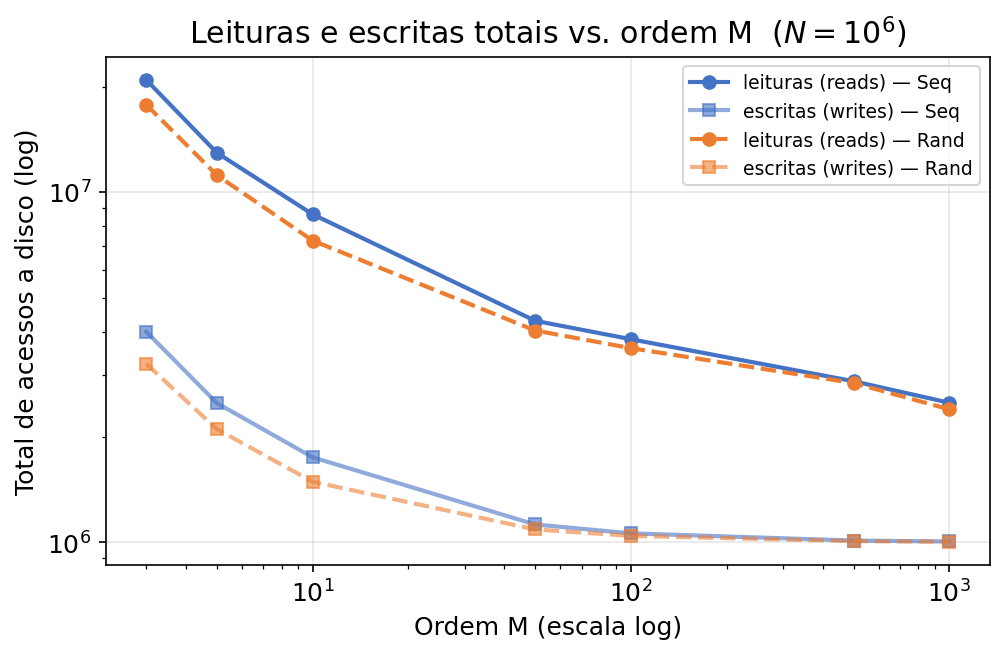
\includegraphics[height=0.74\textheight]{fig_reads_vs_m.png}

  \footnotesize $M\!\uparrow \Rightarrow$ menos \texttt{reads} e \texttt{writes}
  totais (árvore mais rasa: menos nós por inserção). As \texttt{reads} caem de
  ${\sim}21$ para ${\sim}2{,}5$ milhões; \texttt{reads} sempre $>$ \texttt{writes}.
\end{frame}

% ===== Grafico: altura ======================================================
\begin{frame}{Altura da árvore {\small($\times M$ e $\times N$)}}
  \centering
  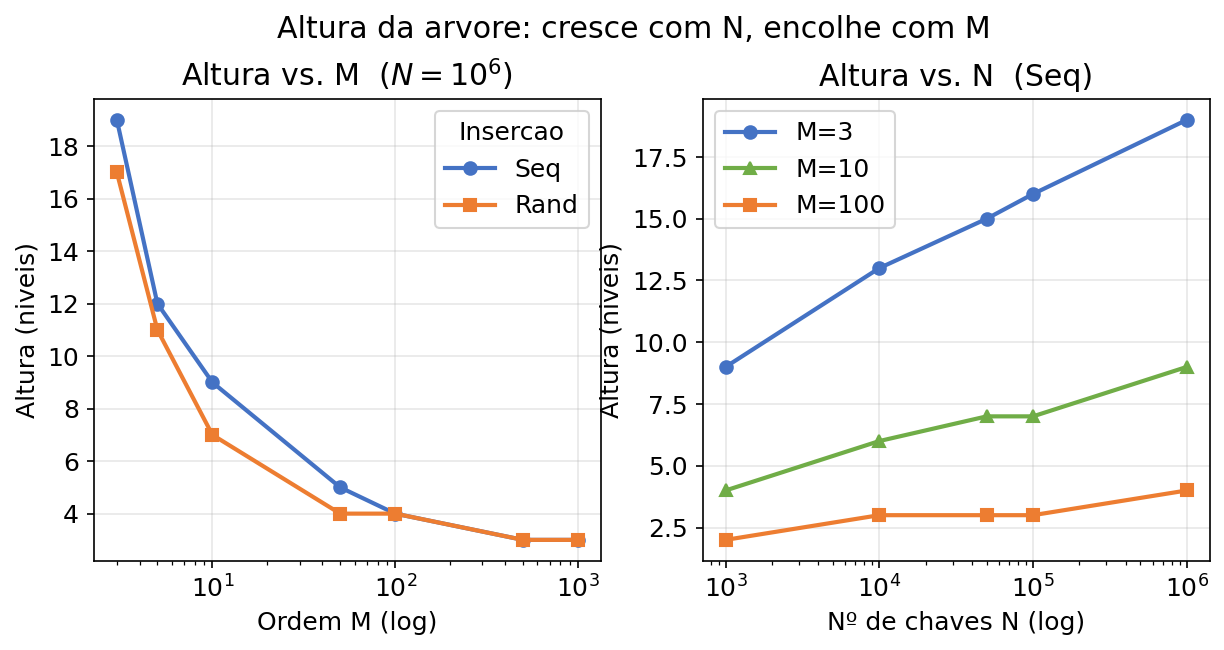
\includegraphics[height=0.74\textheight]{fig_altura.png}

  \footnotesize Altura $\propto \log_M N$: cresce devagar com $N$ e cai
  bruscamente com $M$ (de 19 níveis em $M{=}3$ para 3--4 em $M{\ge}100$, $N{=}10^6$).
\end{frame}

% ===== Grafico: ocupacao Seq vs Rand ========================================
\begin{frame}{Ocupação e padrão de inserção (Seq {\small$\times$} Rand)}
  \centering
  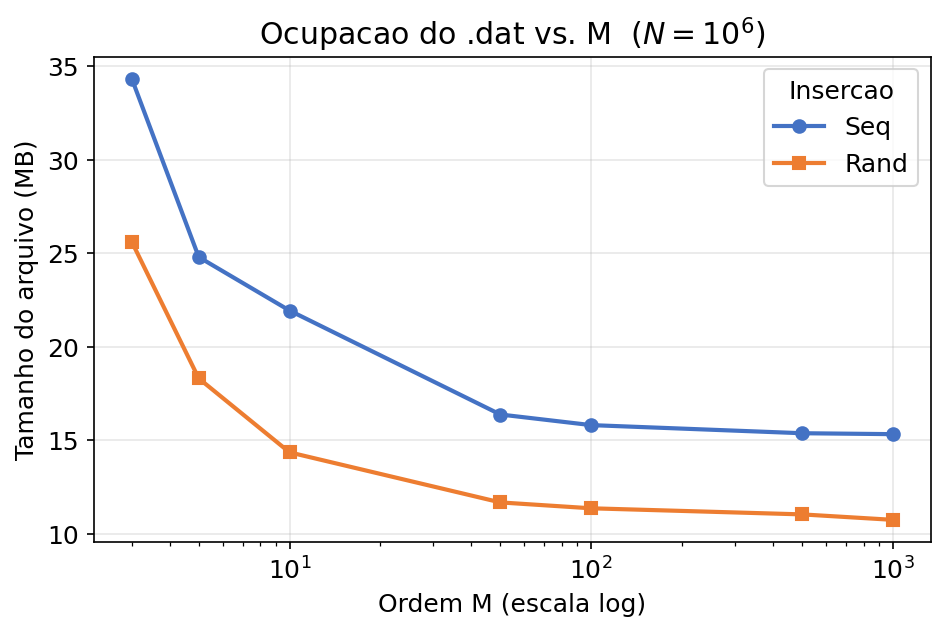
\includegraphics[height=0.72\textheight]{fig_ocupacao.png}

  \footnotesize A inserção \alert{aleatória} preenche melhor os nós (arquivo
  menor); a \alert{sequencial} deixa nós meio-cheios após cada split.
\end{frame}

% ===== Grafico: reuso com vs sem ============================================
\begin{frame}{Reuso de nós: ocupação \emph{com} {\small$\times$} \emph{sem}}
  \centering
  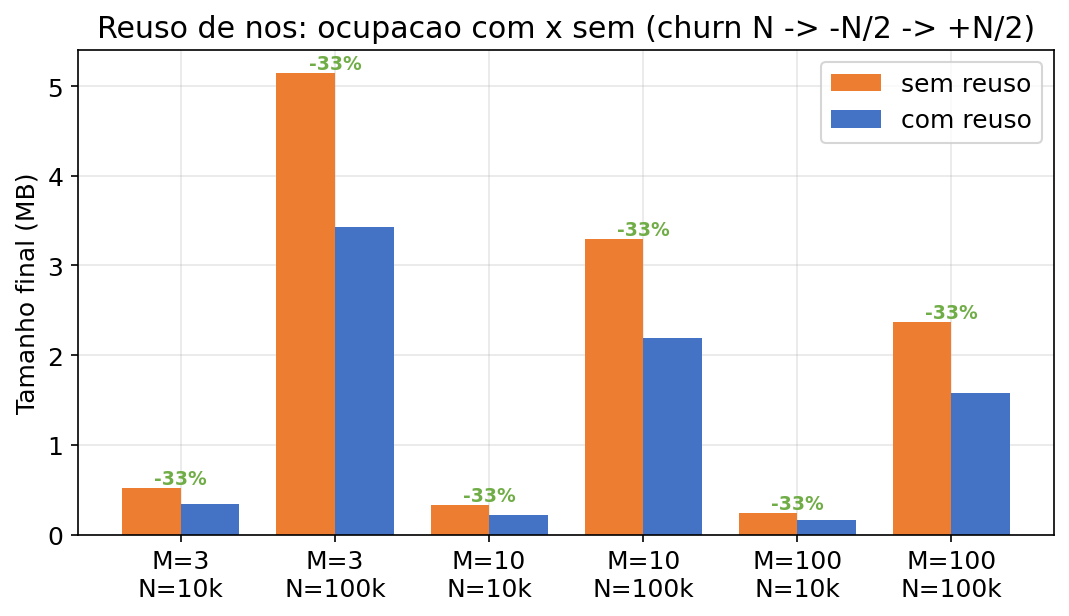
\includegraphics[height=0.72\textheight]{fig_reuso.png}

  \footnotesize \emph{Workload} de \emph{churn} (insere $N$, remove $N/2$,
  reinsere $N/2$): reciclar nós liberados economiza \alert{$\approx$1/3} de disco.
\end{frame}

% ###########################################################################
\section{Discussão}
% ###########################################################################

% ===== Slide 7: Utilizacao de IA ============================================
\begin{frame}{Utilização de IA}
  Usamos um assistente de IA como \alert{apoio}, sempre com validação humana e
  conferência contra os dados e o enunciado. Onde ajudou:
  \vspace{0.2em}
  \begin{description}\footnotesize
    \item[Revisão de código] Revisão crítica que apontou casos de borda ---
      destaque para a \alert{falha silenciosa de I/O} quando \texttt{tmp/} não
      existia.
    \item[Geração de casos de teste] Sugestão de \emph{fixtures} e cenários
      que ampliaram a cobertura para os 27 casos.
    \item[Comentários e documentação] Apoio na redação de comentários do código,
      do \texttt{README} e dos cabeçalhos das funções.
    \item[Revisão dos slides] Conferência da aderência ao modelo do enunciado e
      da consistência dos números com os CSVs.
  \end{description}
  \vspace{0.2em}
\end{frame}

% ===== Slide 10: Conclusao e Referencias ====================================
\begin{frame}{Conclusão e Referências}
  \begin{itemize}
    \item \textbf{Ordem $M$ reduz acessos e altura:} para $10^6$ chaves, as
      \alert{leituras} caem de ${\sim}21$ milhões ($M{=}3$) para ${\sim}2{,}5$
      milhões ($M{=}1000$) e as \alert{escritas} de ${\sim}4{,}0$ para ${\sim}1{,}0$
      milhão; a altura, de \alert{19 para 3} níveis.
    \item \textbf{Cache vs.\ disco real:} os tempos da bateria refletem o
      \alert{page cache} (o \texttt{.dat} cabe na RAM; device NVMe). Forçando I/O
      real por \texttt{cgroup}, só a inserção \alert{aleatória} (baixa localidade)
      paga disco; a \alert{contagem de acessos} (lógica) independe da máquina.
    \item \textbf{Reuso de nós economiza $\approx$33\%} de ocupação do arquivo.
    \item \textbf{Conformidade:} I/O estritamente 1 nó por vez (1 seek + 1 struct).
  \end{itemize}
  \vspace{0.2em}
  \footnotesize\textbf{Referências:} CORMEN et al. \emph{Introduction to
  Algorithms}, 4.\,ed., MIT Press, 2022 (Cap.~18). \,COMER, D. ``The Ubiquitous
  B-Tree''. \emph{ACM Comp. Surveys}, 1979. \,KNUTH, D. \emph{TAOCP}, v.3.
\end{frame}

% ===== Encerramento =========================================================
\begin{frame}[plain]
  \centering\vspace{1.2cm}
  {\usebeamercolor[fg]{title}\Huge\bfseries Obrigado!}\\[1.2em]
  \large Caio Uehara \quad\textbullet\quad Yuri Calzzani \quad\textbullet\quad Igor Felipe
\end{frame}

\end{document}
